\section{Numerical}
\subsection{Methods}
Section \ref{sec:experiments} includes a number of numerical experiments and results. This section explains how we arrived at those results, by showing our programmatic approach to the problem. The code used to solve the optimization problems and to generate the figures can be found in \href{https://github.com/otkulseng/Opt1_Project}{this} Github repository.
\subsubsection{BFGS}
This is a completely generic implementation of the BFGS method in the \href{https://github.com/otkulseng/Opt1_Project/blob/main/Kode/algoritmer.py}{algoritmer.py} file. The implementation follows closely that of algorithm 6.1 in \cite{NW}, the only difference being the choice of steplength. Our implementation uses a line search method to find a steplength that satisfies the \emph{strong} Wolfe conditions, rather than the regular ones used in the book.

The linesearch method is based on algorithm 3.5 in \cite{NW}, with a bisecting interpolation implementation of zoom (algorithm 3.6). The next steplength is chosen according to $\alpha_{k+1} = \rho \alpha_k$. The number $\rho$ together with $c_1$ and $c_2$ completely specify the algorithm, and are preset as
\begin{gather}    
\begin{tabular}{||c c c||} 
 \hline
 $\rho$ & $c_1$ & $c_2$ \\ [0.5ex] 
 \hline
2 & 0.01 & 0.9  \\ 
 \hline
\end{tabular}
\end{gather}
The BFGS iterations stop either when some predetermined maximum iterations has been reached, or when the norm of the gradient is below a threshold of $\num{1e-10}$.

BFGS has been shown to converge under certain assumptions, most notably convexity and the objective function being twice continiously differentiable. The objective functions we consider in this project are not $C^2$, and only \eqref{cableNet} is convex. One could consider applying other methods such as gradient descent as they have better theoretical guarantees of convergence, but they are significantly slower than BFGS. As BFGS is known to work very well in practice, we will exclusively use this algorithm in this project. \textbf{LEST OVER DETTE?}

\subsubsection{Tensegrity}
This is the generation of objective and gradient functions, and can be found in the \href{https://github.com/otkulseng/Opt1_Project/blob/main/Kode/tensegrity.py}{tensegrity.py} file. 

When creating a TensegrityStructure, the functions \lstinline{gen_E}  and \lstinline{gen_grad_E} are called with the corresponding cables, bars, free weights, fixed points and rest lengths and returns the objective and gradient functions of the setup according to the equations in the previous sections. The returned functions take as input only the position of the free points, which are the variables to be optimized. This is neat, as it allows us to use any generic optimization algorithm to solve the problem.

\subsubsection{Freestanding structures}
Instead of solving \eqref{totalEnergy} subject to \eqref{z_positive}, we added quadratic penalization to the energy and gradient functions. The objective function thus gained a term of the from 
\begin{equation}
    E_{qp} = \sum_{i \in \mathcal{N}} \frac{1}{2} \mu (x_3^{(i)})^2
\end{equation}
where $\mathcal{N}$ is the set of all points with z-component smaller than zero. This $\mu$ should be large enough to counteract the gravitational pull on the nodes. To avoid having to modify the BFGS method to account for quadratic penalty, we ran BFGS multiple times for increasing values of $\mu$ like in the code snippet below.

\begin{lstlisting}
prev = x0
for _ in range(Max_iter):
    res, num = bfgs(prev, ts.func(mu), ts.grad(mu), Niter=1000)
    mu *= 1.5
    if num < 1000:
        mu *= 2
    if num < 500:
        mu *= 2
    if num < 250:
        mu *= 2

    mu = min(mu, 1e10)
    if np.linalg.norm(res - prev) < 1e-12:
        break
    prev = res.copy()
\end{lstlisting}
The code snippet above was used for all freestanding structures.

Freestanding structures may be shifted along any vector in the $x_1$ - $x_2$ plane without change in energy, as shown in section \ref{sec:invariance}. The structure may also be rotated around any axis parallel to the $x_3$-axis. These observations affected our convergence. We therefore put three extra constraints on \ref{totalEnergy}:

\begin{equation}
    x_{1}^{(1)} = x_{2}^{(1)} = 0 \textbf{ and } x_{1}^{(1)} = x_{1}^{(2)}
\end{equation}

The first two constraints fix the position of the structure so that one point ends up close to $(0, 0, 0)$. The last one fixes the orientation of the structure, by requiring that two neigboring points share the same $x_1$ value. We should only do this with structures having at least two points on the ground. 
 
\subsection{Experiments}\label{sec:experiments}
The setup for all numerical experiments may be found in the \href{https://github.com/otkulseng/Opt1_Project/blob/main/Kode/tests.py}{tests.py} file. The Tensegrity structure setup is also for convenience given below, before every experiment.
\subsubsection{Cable nets}
For the first experiment we will consider $4$ free and $4$ fixed nodes along with the following parameters:
\begin{equation*}
\begin{gathered}
    4 \text{ fixed nodes } p^{(1)} = (5,5,0),\; p^{(2)} = (-5,5,0),\; p^{(3)} = (-5,-5,0),\; p^{(4)} = (5,-5,0) \\
    \text{Cables: } \ell_{15} = \ell_{26} = \ell_{37} = \ell_{48} = \ell_{56} = \ell_{67} = \ell_{78} = \ell_{85} = 3\\ 
    k = 3, \quad m_i g = \frac{1}{6}, \quad i= 5,6,7,8 
\end{gathered}
\end{equation*}

We will initialise the free nodes with a random node placement. This problem has a analytical solution which is given in \eqref{P25Table} along with the numerically obtained solution. 

\begin{figure}    
\caption{Comparison of numerical and analytical solution for the cable net.}
\label{P25Table}
\begin{gather}
\begin{tabular}{||c c c||} 
    \hline
    Node & Numerical solution & Analytical solution \\ [0.5ex] 
    \hline
    $x^{(5)}$ & $(2,2,-1.5)$ & $(2,2,-1.5)$  \\ 
    \hline
    $x^{(6)}$ & $(-2,2,-1.5)$& $(-2,2,-1.5)$  \\ 
    \hline
    $x^{(7)}$ & $(-2,-2,-1.5)$ & $(-2,-2,-1.5)$\\ 
    \hline
    $x^{(8)}$ & $(2,-2,-1.5)$ & $(2,-2,-1.5)$ \\ 
    \hline
\end{tabular}
\end{gather}
\end{figure}



\begin{figure}[!ht]
\centering
\begin{subfigure}{.72\textwidth}
  \centering
  \includegraphics[width=0.99\linewidth]{Bilder/p25.pdf}
\end{subfigure}%
\begin{subfigure}{.3\textwidth}
  \centering
  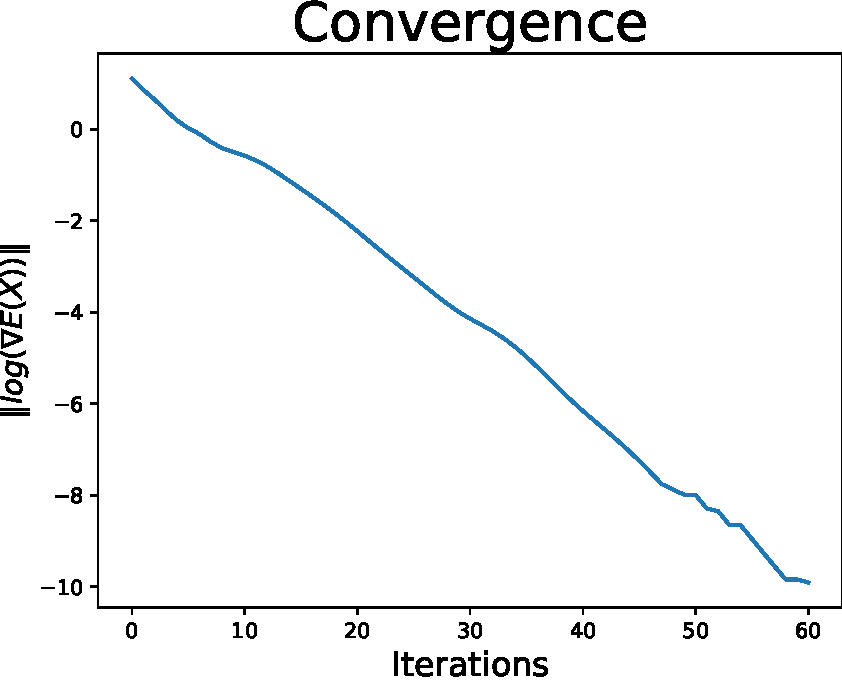
\includegraphics[width=0.99\linewidth]{Bilder/P25conv.pdf}
\end{subfigure}
\caption{Cable net. Left: Randomized initial node placement. Centre left: Solution. Centre right: Solution from a different viewpoint. Right: Convergence plot.}
\label{P25}
\end{figure}

We see from figure \ref{P25} that we indeed reach this configuration of nodes. We see from the convergence plot that the gradient never increases, presumably a consequence of the function being convex. \textbf{Hadde vært nice å ha noe mer konkret å vise til her, men tror ikke det finnes noe..?}
\textbf{HVIS VI ENDRER CONV-PLOT MÅ DETTE ENDRES} 

\subsubsection{Tensegrity domes}
We now consider bars as well. The objective function is no longer convex. As discussed previously, $E(X)$ is technically not $C^1$, but as long as we do not initialize free nodes in the same position, it will be fine in practice. We will test our algorithm with $4$ fixed nodes and the following parameters:
\begin{equation*}
    \begin{gathered}
    p^{(1)} = (1,1,0),\; p^{(2)} = (-1,1,0),\; p^{(3)} = (-1,-1,0),\; p^{(4)} = (1,-1,0)\\
    \text{Cables: } \ell_{18} = \ell_{25} = \ell_{36} = \ell_{47} = 8, \qquad \ell_{56} = \ell_{67} = \ell_{78} = \ell_{58} = 1\\
    \text{Bars: }\ell_{15} = \ell_{26} = \ell_{37} = \ell_{48} = 10\\
    c=1, \quad k= 0.1, \quad g \rho = 0,\quad m_i g = 0, \quad i = 5,6,7,8
    \end{gathered}
\end{equation*}

We have an analytical solution to this problem, a comparison is given in \eqref{P69Table}. 
\begin{figure}
\caption{Comparison of numerical and analytical solution for the cable net}
\begin{gather}   
\label{P69Table}
\begin{tabular}{||c c c||} 
 \hline
 Node & Numerical solution & Analytical solution \\ [0.5ex] 
 \hline
$x^{(5)}$ & $(0.70971,2.30372 \cdot 10^{-8},9.54287)$ & $(-0.70970,0,9.54287)$  \\ 
 \hline
 $x^{(6)}$ & $(6.70558 \cdot 10^{-9},-0.70971,9.54287)$& $(0,-0.70970,9.54287)$  \\ 
 \hline
 $x^{(7)}$ & $(0.70970,2.98982 \cdot 10^{-8},9.54287)$ & $(0.70970,0,9.54287)$\\ 
 \hline
 $x^{(8)}$ & $(5.14925 \cdot 10^{-10},0.70970,9.54287)$ & $(0,0.70970,9.54287)$ \\ 
 \hline
\end{tabular}
\end{gather}
\end{figure}

\begin{figure}[!ht]
\centering
\begin{subfigure}{.72\textwidth}
  \centering
  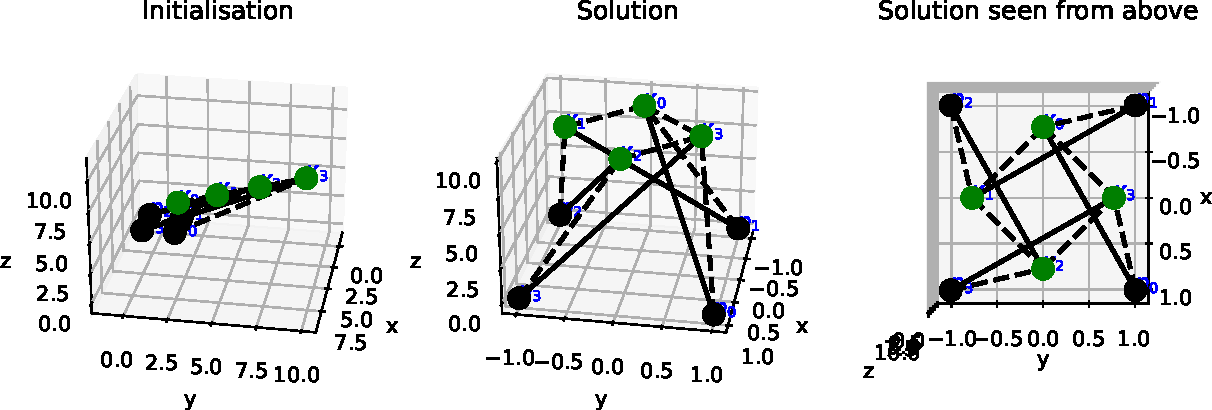
\includegraphics[width=0.99\linewidth]{Bilder/P69.pdf}
\end{subfigure}%
\begin{subfigure}{.3\textwidth}
  \centering
  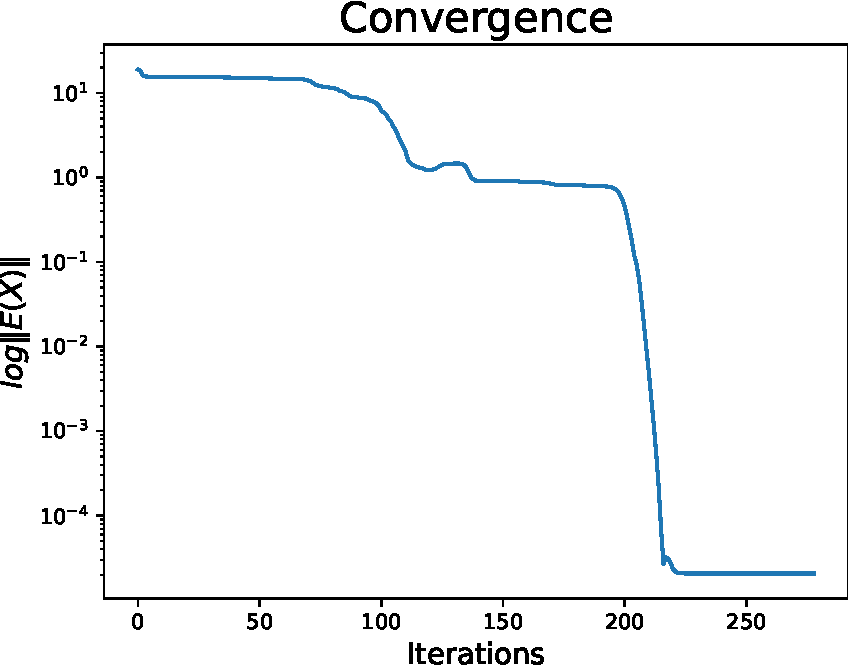
\includegraphics[width=0.99\linewidth]{Bilder/P69conv.pdf}
\end{subfigure}
\caption{Tensegrity dome. Left: Randomized initial node placement. Centre left: Solution. Centre right: Solution from a different viewpoint. Right: Convergence plot.}
\label{P69}
\end{figure}

Again, we see from \eqref{P69} that we reach the desired configuration of nodes from our randomized initial node placement. 


As for the free standing structure, we will consider a configuration fairly close to the Tensegrity dome in order to verify the results. We use the same parameters, but in addition we add the cables 
$\ell_{12} = \ell_{23} = \ell_{34} = \ell_{41} = 2 $ and use a small positive value of $\rho = 10^{-10}$

\begin{figure}[!ht]
\centering
\begin{subfigure}{.72\textwidth}
  \centering
  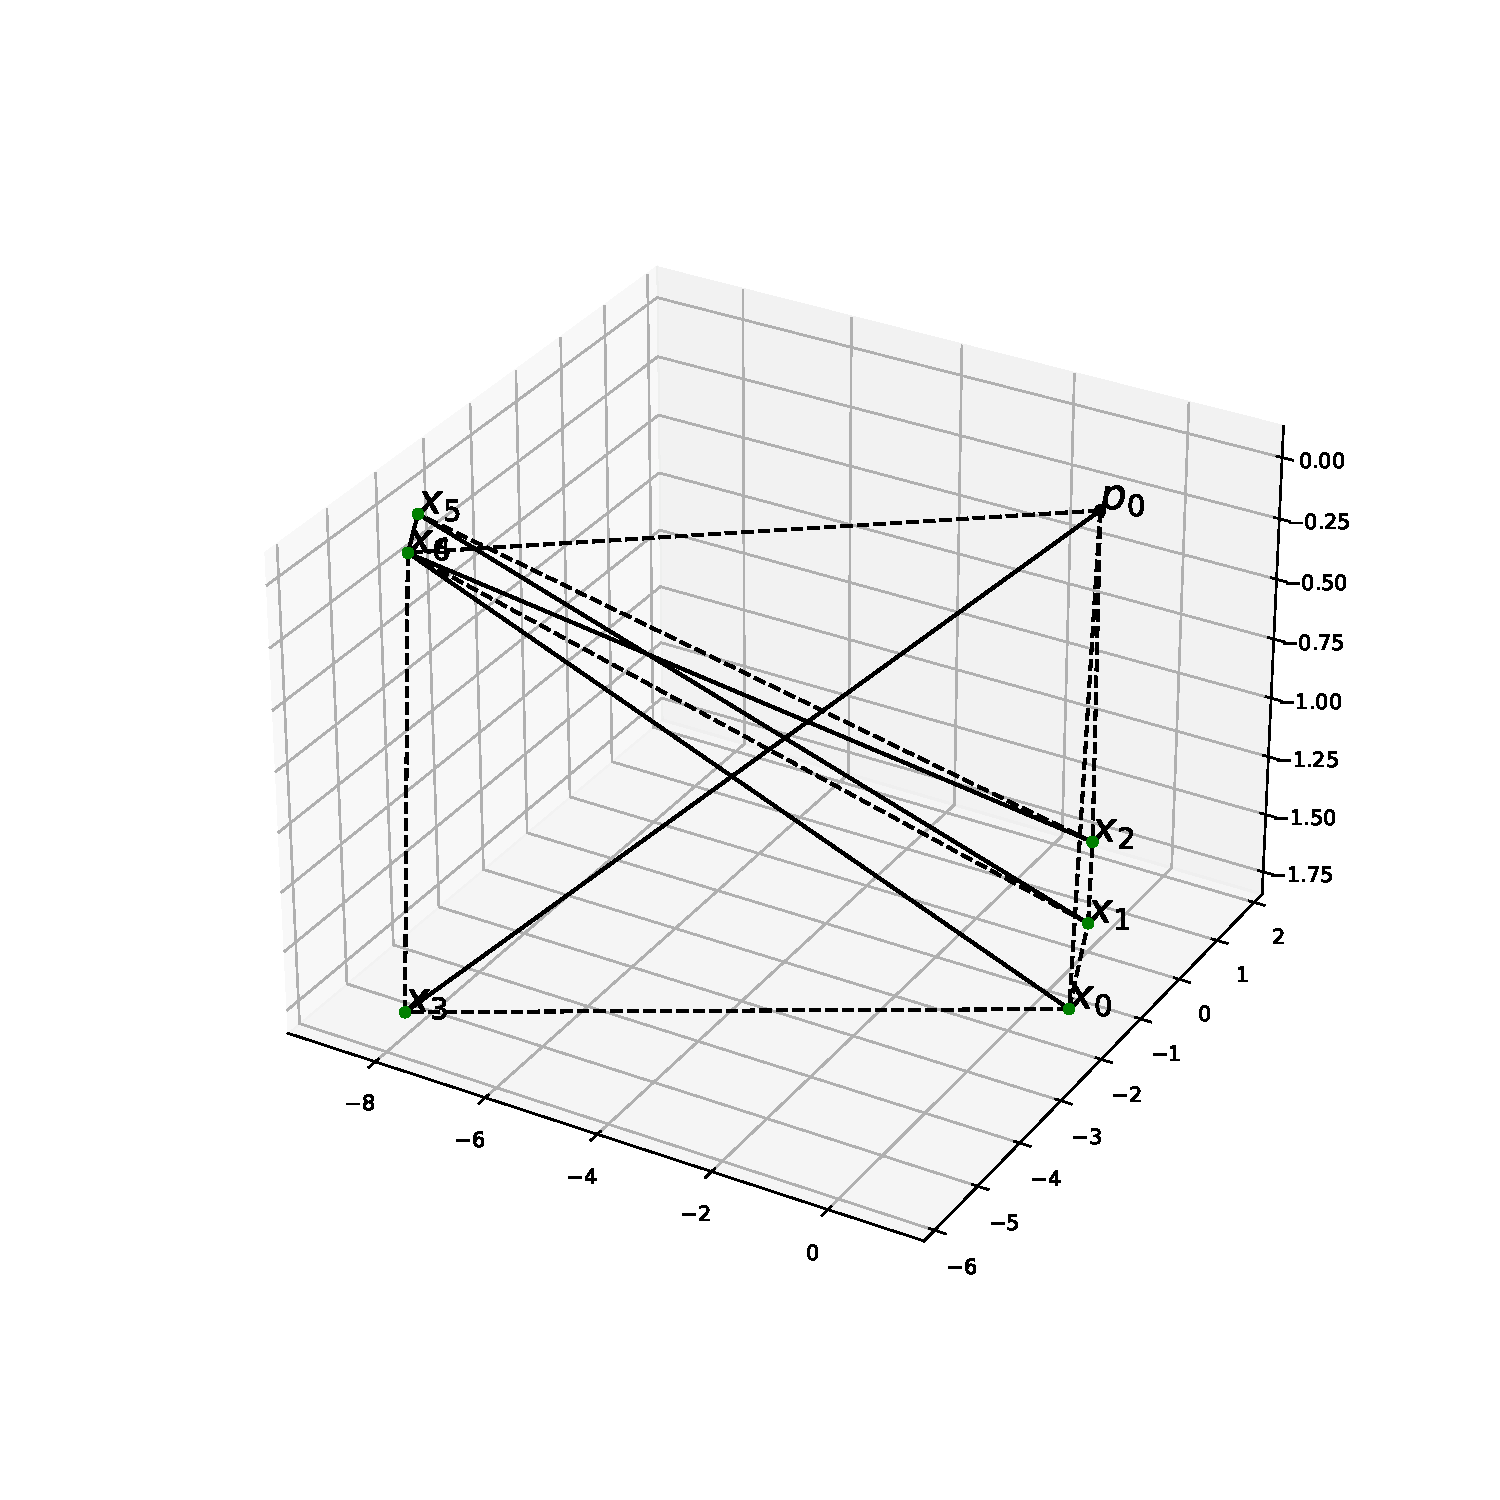
\includegraphics[width=0.99\linewidth]{Bilder/FREESTANDING.pdf}
\end{subfigure}%
\begin{subfigure}{.3\textwidth}
  \centering
  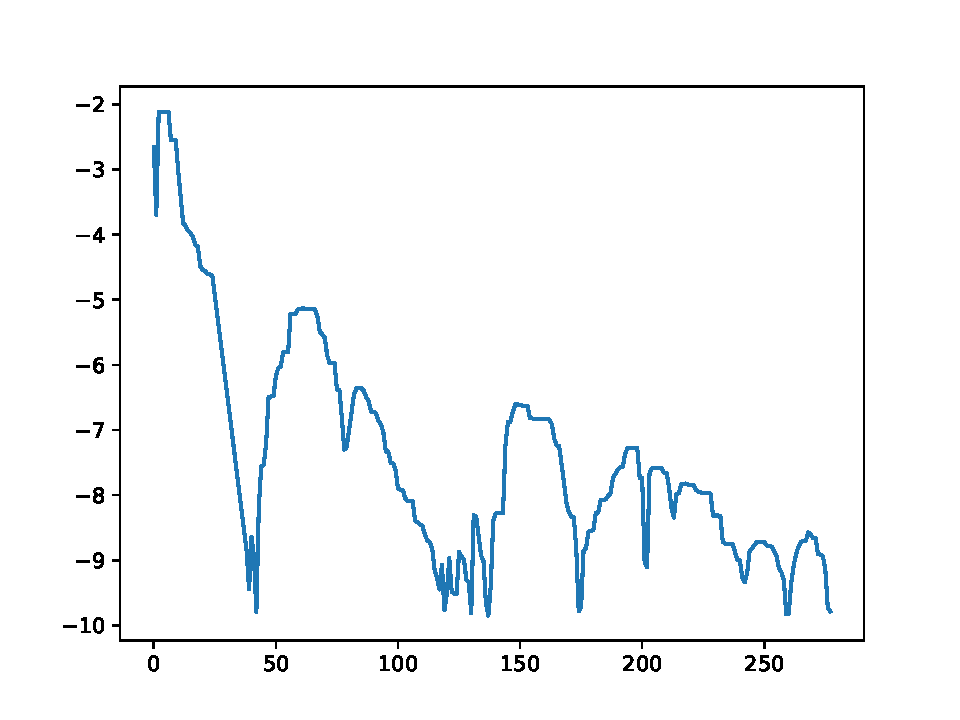
\includegraphics[width=0.99\linewidth]{Bilder/FREESTANDINGconv.pdf}
\end{subfigure}
\caption{Free standing tensegrity dome. Left: Randomized initial node placement. Centre left: Solution. Centre right: Solution from a different viewpoint. Right: Convergence plot.}
\label{Freestanding}
\end{figure}



\begin{figure}[!ht]
\centering
\begin{subfigure}{.72\textwidth}
  \centering
  \includegraphics[width=0.99\linewidth]{Bilder/2FREESTANDING.pdf}
\end{subfigure}%
\begin{subfigure}{.3\textwidth}
  \centering
  \includegraphics[width=0.99\linewidth]{Bilder/2FREESTANDINGconv.pdf}
\end{subfigure}
\caption{Two free standing tensegrity domes stacked on top of eachothers. Left: Randomized initial node placement. Centre left: Solution. Centre right: Solution from a different viewpoint. Right: Convergence plot.}
\label{2free}
\end{figure}